\section{Auswertung}
\label{sec:Auswertung}

\subsection{Bestimmung der Winkelrichtgröße}

Die Messung wird mit einem senkrechten Abstand von ${r=\SI{4.0}{\centi\meter}}$ durchgeführt. 
Der Auslenkwinkel $\varphi$ und die aufgewendete Kraft $F$ sind in \ref{tab:richtgrD} dargestellt, ebenso wie die sich daraus 
ergebenden Werte für die Winkelrichtgröße $D$. 
Sie berechnet sich, wie aus der Theorie zu entnehmen ist, über 
\begin{equation}
    D=\frac{Fr}{\varphi}\:.
\end{equation}

\begin{table}
    \centering
    \caption{Messwerte zur Bestimmung der Winkelrichtgröße.}
    \label{tab:richtgrD}
    \begin{tabular}{c S[table-format=1.2] S[table-format=1.2] S[table-format=2.1]}
        \toprule
        {$\varphi$} & {$\varphi\:/\:\symup{\pi}$} & {$F\:/\:\si{\newton}$} & {$D\:/\:\SI{e-3}{\newton\meter}$} \\
        \midrule
        \ang{26;;}  & 0.14  & 0.19 & 17.3 \\
        \ang{30;;}  & 0.17  & 0.21 & 15.7 \\
        \ang{37;;}  & 0.21  & 0.29 & 17.6 \\
        \ang{45;;}  & 0.25  & 0.41 & 20.9 \\
        \ang{60;;}  & 0.33  & 0.49 & 18.9 \\
        \ang{70;;}  & 0.39  & 0.61 & 19.9 \\
        \ang{81;;}  & 0.45  & 0.70 & 19.8 \\
        \ang{93;;}  & 0.52  & 0.74 & 18.1 \\
        \ang{100;;} & 0.56  & 0.91 & 20.7 \\
        \ang{110;;} & 0.61  & 0.97 & 20.2 \\
        \bottomrule
    \end{tabular}
\end{table}

Somit ergibt sich als experimenteller Wert ${D=\SI{18.9\pm1.6e-3}{\newton\meter}}$ für die Winkelrichtgröße. 
Die Abweichung der Größe berechnet sich über 
\begin{equation}
    \increment D = \sqrt{\frac{1}{N-1}\sum_{i=1}^N (D_i-\bar{D})^2}
    \label{eqn:fehler}
\end{equation}
mit dem arithmetischen Mittel $\bar{D}$. 

\FloatBarrier
\subsection{Bestimmung des Eigenträgheitsmoments der Drillachse}

Im Folgenden sei die Annahme eines nahezu masselosen Stabs, an dem zwei Punktmassen -- demnach ohne Ausdehnung -- 
gleicher Masse ${m=\SI{222.89}{\gram}}$ 
befestigt sind. 
In \ref{tab:I_D} sind die Messwerte entsprechend dargestellt. 
Es besteht ein linearer Zusammenhang zwischen den Quadraten der Periode $T$ und dem Abstand $a$ der Massen:

\begin{equation}
    T^2=\frac{4\symup{\pi}^2}{D}\bigl(I_\text{D} + m(a_1^2+a_2^2)\bigr)=:\frac{4\symup{\pi}^2}{D}(I_\text{D}+ma^2)    
    \label{eqn:Thoch2}
\end{equation} 

\begin{table}
    \centering
    \caption{Messwerte zur Bestimmung des Eigenträgheitsmoments $I_\text{D}$.}
    \label{tab:I_D}
    \begin{tabular}{S[table-format=2.1] S[table-format=2.1] S[table-format=4.1] S[table-format=1.2] S[table-format=2.2]}
        \toprule
        {$a_1\:/\:\si{\centi\meter}$} & {$a_2\:/\:\si{\centi\meter}$} & {$(a_1^2+a_2^2)\:/\:\si{\centi\meter\squared}$} & {$T\:/\:\si{\second}$} & {$T^2\:/\:\si{\second\squared}$} \\
        \midrule
        4.5  & 5.5  &   50.5 & 2.50 & 6.25  \\
        6.5  & 7.5  &   98.5 & 2.93 & 8.58  \\
        8.5  & 9.5  &  162.5 & 3.21 & 10.30 \\
        10.5 & 11.5 &  242.5 & 3.83 & 14.67 \\
        12.5 & 13.5 &  338.5 & 4.16 & 17.31 \\
        14.5 & 15.5 &  450.5 & 4.70 & 22.09 \\
        16.5 & 17.5 &  578.5 & 5.27 & 27.77 \\
        18.5 & 19.5 &  722.5 & 5.79 & 33.52 \\
        20.5 & 21.5 &  882.5 & 6.27 & 39.31 \\
        22.5 & 23.5 & 1058.5 & 6.78 & 45.97 \\
        \bottomrule
    \end{tabular}
\end{table}

Nun werden diese Werte in einem Diagramm aufgetragen. 
Mithilfe linearer Regression lässt sich aus dem Y-Achsenabschnitt $b$ das Eigenträgheitsmoment $I_D$ bestimmen. 
Die Steigung $c$ ergibt sich unter Vergleich mit \eqref{eqn:Thoch2} aus

\begin{gather}
y=b+cx \\
T^2 = \frac{4\symup{\pi}^2}{D}(I_\text{D}+ma^2) \\
\Rightarrow y = T^2, 
\quad b =  \frac{4\symup{\pi}^2}{D} I_\text{D}, 
\quad c = \frac{4\symup{\pi}^2}{D}m ,
\quad x = a^2 
\end{gather}

Unter Zuhilfenahme von \texttt{Python 3.7.3} wird die lineare Regression durchgeführt, wie in Abbildung \ref{fig:Thoch2} zu sehen ist, und es ergibt sich der y-Achsenabschnitt~${b=\SI{4.42(25)}{\second\squared}}$
und eine Steigung von ${c=\SI{396.0\pm4.4}{\kilo\gram\per\joule}}$. 
Daraus lässt sich das Eigenträgheitsmoment zu 
\begin{equation}
    I_\text{D}=\frac{D}{4\symup{\pi}^2}b=\frac{m}{c}b=\SI{2.49(14)e-3}{\kilo\gram\meter\squared}
\end{equation}
bestimmen.

\begin{figure}
    \centering
    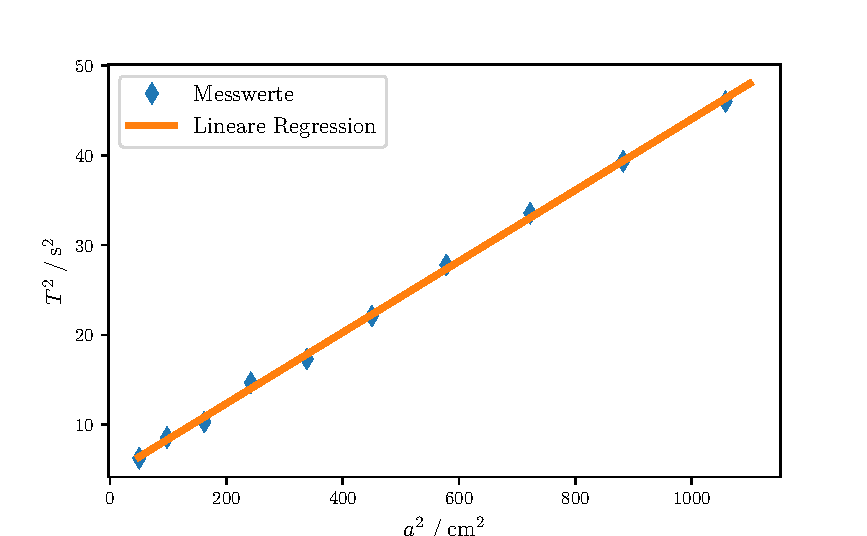
\includegraphics[width=0.8\textwidth]{plots/plot_I_D.pdf}
    \caption{Lineare Regression zur Bestimmung des Eigenträgheitsmoments.}
    \label{fig:Thoch2}
\end{figure}

\FloatBarrier
\subsection{Trägheitsmomente verschiedener Körper}

In den Tabellen \ref{tab:messSchwing} und \ref{tab:mittelSchwing} sind die Messwerte aufgetragen, die zur Bestimmung der 
Trägheitsmomente zweier verschiedener Zylinder und einer Holzpuppe in zwei unterschiedlichen Posen aufgenommen worden sind. 
In \ref{tab:mittelSchwing} berechnet sich der Messfehler ebenfalls über \eqref{eqn:fehler}. 

\begin{figure}
    \centering
    \begin{subfigure}{0.48\textwidth}
        \centering
        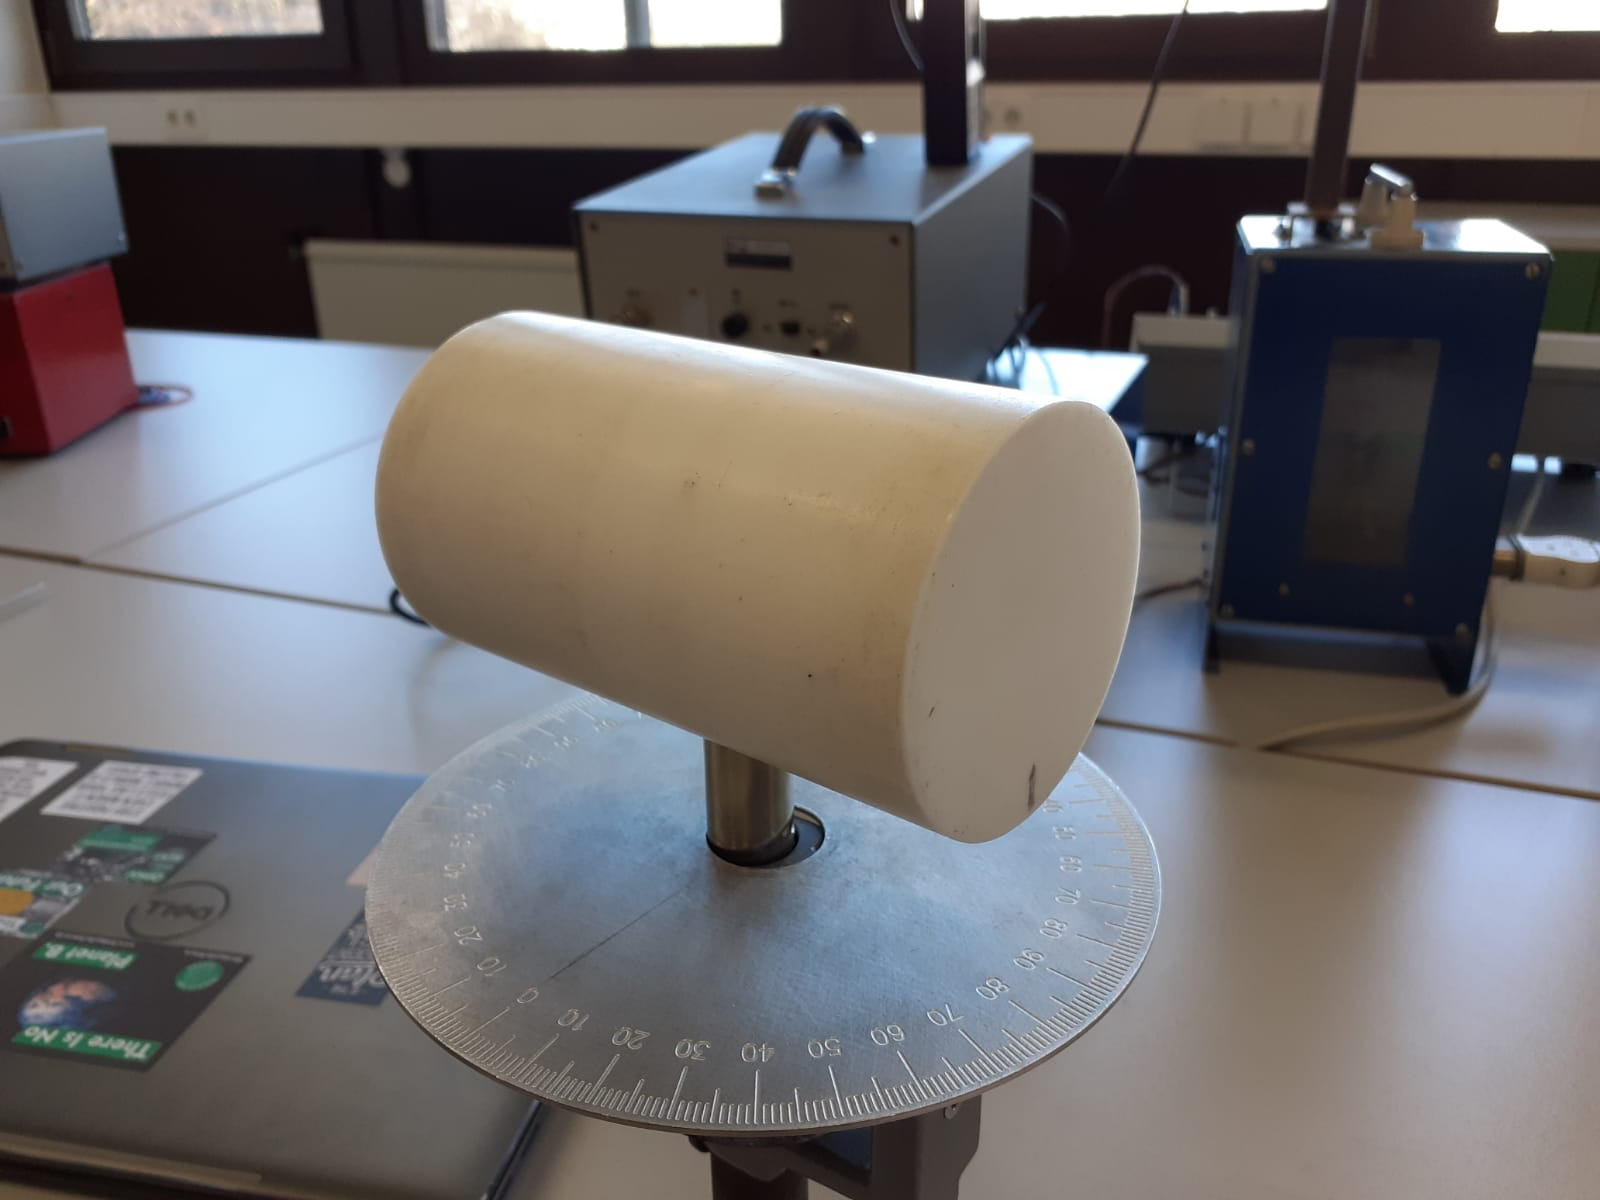
\includegraphics[height=5cm]{plots/Zyl_big.jpeg}
        \caption{Der große Zylinder.}
        \label{fig:grZyl}
    \end{subfigure}
    \begin{subfigure}{0.48\textwidth}
        \centering
        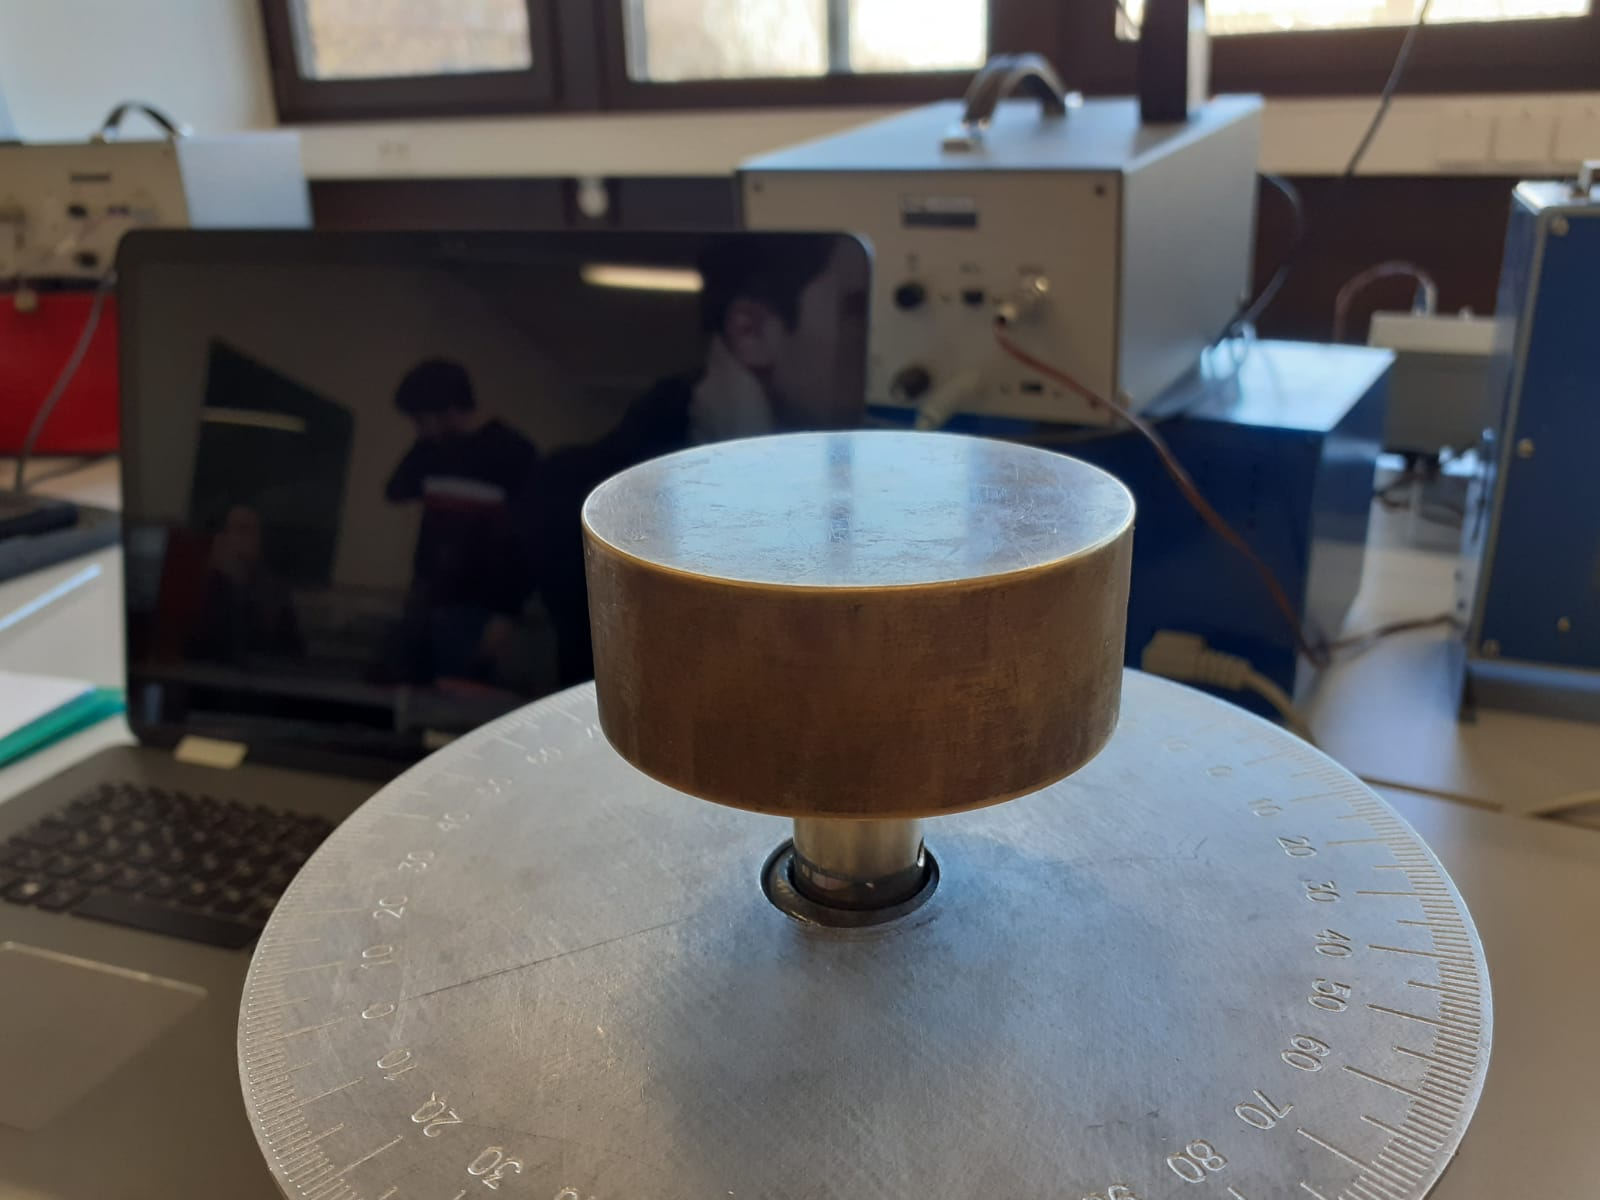
\includegraphics[height=5cm]{plots/Zyl_small.jpeg}
        \caption{Der kleine Zylinder.}
        \label{fig:klZyl}
    \end{subfigure}
    \caption{Die verwendeten Zylinder und ihre Drehachsen im Experiment.}
    \label{fig:Zyl}
\end{figure}

\begin{figure}
    \centering
    \begin{subfigure}{0.48\textwidth}
        \centering
        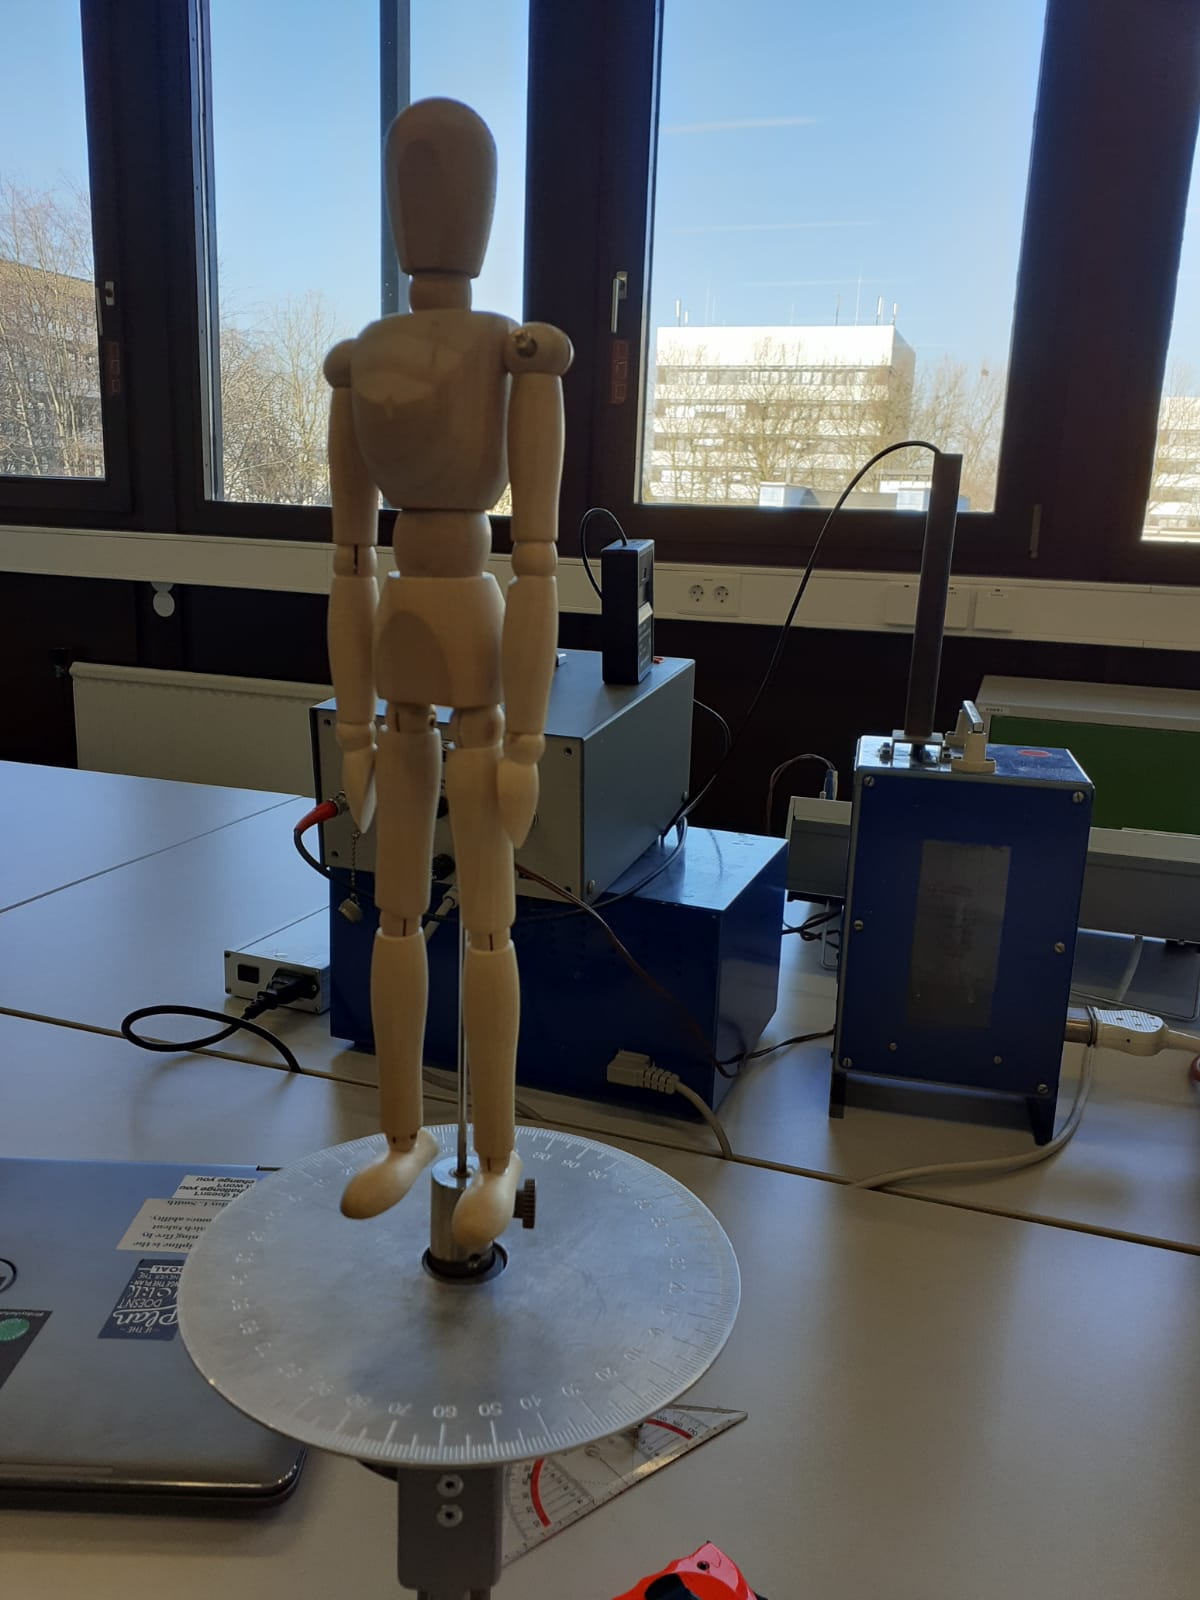
\includegraphics[height=5cm]{plots/figur1.jpeg}
        \caption{Pose 1.}
        \label{fig:pos1}
    \end{subfigure}
    \begin{subfigure}{0.48\textwidth}
        \centering
        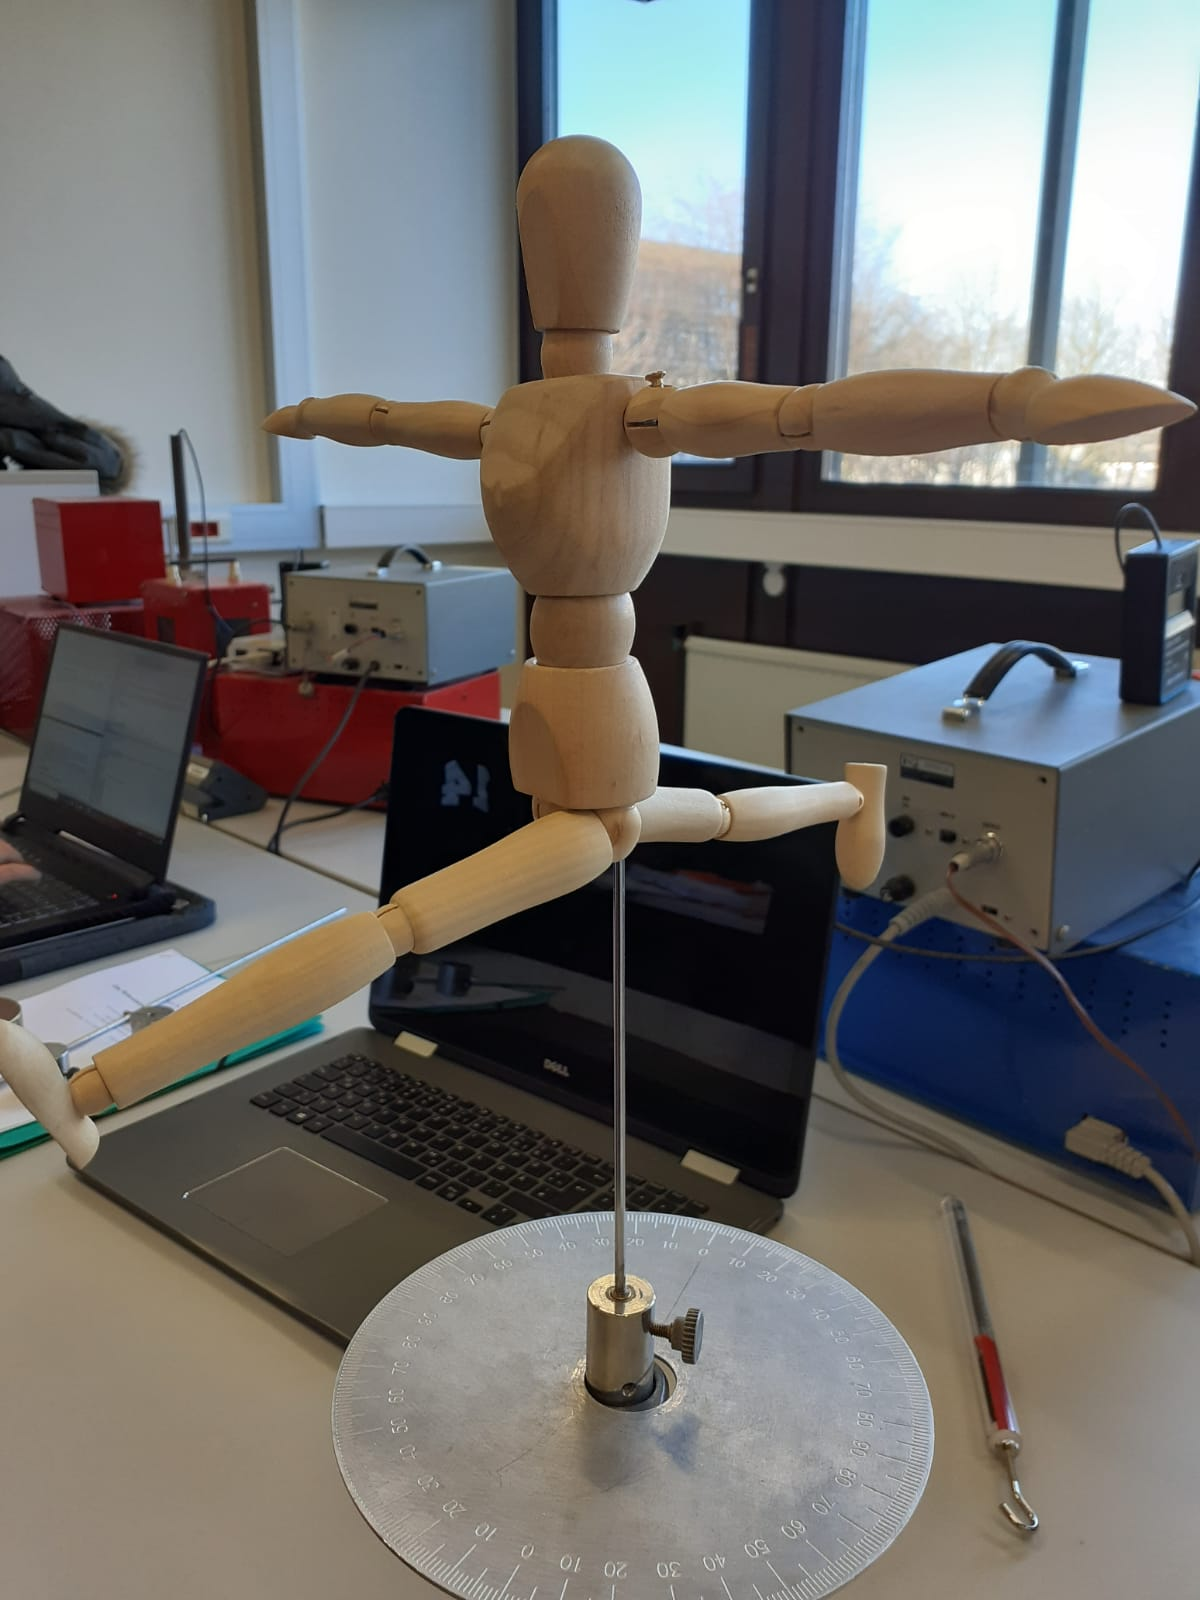
\includegraphics[height=5cm]{plots/figur2.jpeg}
        \caption{Pose 2.}
        \label{fig:pos2}
    \end{subfigure}
    \caption{Die Holzpuppe in zwei verschiedenen Stellungen.}
    \label{fig:puppe}
\end{figure}

\begin{table}
    \centering
    \caption{Messwerte aller Schwingungsdauern.}
    \label{tab:messSchwing}
    \begin{tabular}{c c c c}
        \toprule
        {$T_\text{Zyl,groß}\:/\:\si{\second}$} & {$T_\text{Zyl,klein}\:/\:\si{\second}$} & {$T_\text{Pose1}\:/\:\si{\second}$} & {$T_\text{Pose2}\:/\:\si{\second}$} \\
        \midrule
        1.08 & 2.31 & 0.38 & 0.92 \\
        1.27 & 2.23 & 0.41 & 0.89 \\
        1.13 & 2.17 & 0.43 & 0.94 \\
        1.18 & 2.30 & 0.39 & 0.91 \\
        1.16 & 2.26 & 0.41 & 0.91 \\
        \bottomrule
    \end{tabular}
\end{table}

\begin{table}
    \centering
    \caption{Messunsicherheiten aller Schwingungsdauern.}
    \label{tab:mittelSchwing}
    \begin{tabular}{l c}
        \toprule
        & {T$\:/\:\si{\second}$} \\     % werden Messgrößen kursiv geschrieben? (hier das T)
        \midrule
        großer Zylinder  & $\SI{2.25(5)}{}$ \\
        kleiner Zylinder  & $\SI{1.16(6)}{}$ \\
        Holzfigur Pose 1  & $\SI{0.40(2)}{}$ \\
        Holzfigur Pose 2  & $\SI{0.91(2)}{}$ \\
        \bottomrule
    \end{tabular}
\end{table}

\FloatBarrier
\subsubsection{Der kleine Zylinder}

\begin{table}
    \centering
    \caption{Maße des kleinen Zylinders und der zugehörigen Halterung.}
    \label{tab:kleZyl}
    \begin{tabular}{c c}
        \toprule
        \multicolumn{2}{c}{Zylinder} \\
        \midrule
        $m$ & \SI{1119.4}{\gram} \\
        $h$ & \SI{3.0}{\centi\meter} \\
        $d$ & \SI{7.45}{\centi\meter} \\
        \bottomrule
    \end{tabular}
    \qquad \qquad 
    \begin{tabular}{c c}
        \toprule
        \multicolumn{2}{c}{Halterung}\\
        \midrule
        $h$ & \SI{1.8}{\centi\meter} \\
        $d$ & \SI{0.6}{\centi\meter} \\
        \bottomrule
            \\
    \end{tabular}
\end{table}

Das erwartete Trägheitsmoment anhand der geometrischen Abmessungen ist 
\begin{gather}
    m_\text{ges}=\SI{1119.4}{\gram}\:, \qquad 
    m_\text{Zyl}=m_\text{ges}\frac{d_\text{Zyl}^2h_\text{Zyl}}{d_\text{Zyl}^2h_\text{Zyl}+d_\text{Halt}^2h_\text{Halt}}=\SI{1115.1}{\gram} \\
    m_\text{Halt} = m_\text{ges}-m_\text{Zyl}=\SI{4.3}{\gram} \\
    I_\text{kl,geo}=\frac{1}{2}m_\text{Zyl}\frac{d_\text{Zyl}^2}{4}+\frac{1}{2}m_\text{Halt}\frac{d_\text{Halt}^2}{4}=\SI{7.74}{\kilo\gram\centi\meter\squared}\:.
\end{gather}

Wird hingegen die gemittelte Periode und die Winkelrichtgröße inklusive der Messfehler verwendet, um über 
\begin{equation}
    T=2\symup{\pi}\sqrt{\frac{I}{D}}
\end{equation}
das Trägheitsmoment zu berechnen, ergibt sich 
\begin{equation}
    I'_\text{kl,T}=T^2\frac{D}{4\symup{\pi}^2}=\SI{6.44(55)}{\kilo\gram\centi\meter\squared}\:.
\end{equation}

Von diesem Wert müsste eigentlich noch das Trägheitsmoment der Drillachse von ${I_\text{D}=\SI{24.9+-1.4}{\kilo\gram\centi\meter\squared}}$ 
abgezogen werden. Da sich für diesen Fall jedoch ein negativer Wert für den kleinen Zylinder ergeben würde und dies 
unphysikalisch ist, kann es sich hierbei nur um einen Messfehler handeln. 

\FloatBarrier
\subsubsection{Der große Zylinder}

Dasselbe Verfahren wird nun für den großen Zylinder angewendet, mit dem Unterschied, dass die Drehachse hier senkrecht zur 
Symmetrieachse des Zylinders steht und deshalb eine etwas abgewandelte, in der Theorie erläuterte Formel verwendet wird. 

\begin{table}
    \centering
    \caption{Maße des großen Zylinders und der zugehörigen Halterung.}
    \label{tab:groZyl}
    \begin{tabular}{c c}
        \toprule
        \multicolumn{2}{c}{Zylinder}\\
        \midrule
        $m$ & \SI{1525.6}{\gram} \\
        $h$ & \SI{13.95}{\centi\meter} \\
        $d$ & \SI{7.95}{\centi\meter} \\
        \bottomrule
    \end{tabular}
    \qquad \qquad 
    \begin{tabular}{c c}
        \toprule
        \multicolumn{2}{c}{Halterung}\\
        \midrule
        $h$ & \SI{1.4}{\centi\meter} \\
        $d$ & \SI{0.55}{\centi\meter} \\ 
        \bottomrule
            \\
    \end{tabular}
\end{table}

\begin{gather}
    m_\text{ges}=\SI{1525.6}{\gram}\:, \qquad 
    m_\text{Zyl}=m_\text{ges}\frac{d_\text{Zyl}^2h_\text{Zyl}}{d_\text{Zyl}^2h_\text{Zyl}+d_\text{Halt}^2h_\text{Halt}}=\SI{1524.9}{\gram} \\
    m_\text{Halt} = m_\text{ges}-m_\text{Zyl}=\SI{0.7}{\gram} \\
    I_\text{gr,geo}=m_\text{Zyl} \Bigl( \frac{d_\text{Zyl}^2}{16} + \frac{h_\text{Zyl}^2}{12} \Bigr) 
        +\frac{1}{2}m_\text{Halt}\frac{d_\text{Halt}^2}{4}=\SI{30.75}{\kilo\gram\centi\meter\squared}
\end{gather}

\begin{gather}
    I'_\text{gr,T}=T^2\frac{D}{4\symup{\pi}^2}=\SI{24.24\pm2.32}{\kilo\gram\centi\meter\squared} 
\end{gather}

Auch hier ergibt sich nach Abzug des Eigenträgheitsmoments ein negativer, unphysikalischer Wert für das Trägheitsmoment. 

\FloatBarrier
\subsubsection{Die Holzpuppe in der ersten Pose}

Zuerst wird das sich aus der Periodendauer ergebende Trägheitsmoment wie bei den Zylindern berechnet: 
\begin{gather}
    I'_\text{P1,T}=T^2\frac{D}{4\symup{\pi}^2}=\SI{0.77(10)}{\kilo\gram\centi\meter\squared} \\
    I_\text{P1,T}=I'_\text{P1,T}-I_\text{D} <0 
\end{gather}

Nun wird anhand geometrischer Annäherungen das Trägheitsmoment bestimmt; die zugehörigen Formeln für Volumina und ihre 
Trägheitsmomente sind in~\ref{sub:Trägheitsmoment} zu finden. 
Die Masse der Puppe beläuft sich auf einen Wert von ${m=\SI{116.29}{\gram}}$. 
Die Beine werden als je zwei Zylinder -- Ober- und Unterschenkel -- mit einem Abstand von etwa 
${a_\text{Beine}=\SI{1.25}{\centi\meter}}$ zwischen Dreh- und Symmetrieachse angenähert.  

\begin{gather}
    l_\text{Ober}=\SI{6.0}{\centi\meter} \quad \quad
    d_\text{Ober}=\SI{1.8}{\centi\meter} \quad \quad
    V_\text{Ober}=\SI{15.3}{\centi\meter\tothe{3}} \\
    l_\text{Unter}=\SI{7.0}{\centi\meter} \quad \quad
    d_\text{Unter}=\SI{1.6}{\centi\meter} \quad \quad
    V_\text{Unter}=\SI{14.1}{\centi\meter\tothe{3}} 
\end{gather}

Die Füße werden als zwei liegende, entlang der Symmetrieachse durchgeschnitte Zylinder betrachtet, die den gleichen 
Abstand zur Drehachse wie die Beine haben: ${a_\text{Füße}=a_\text{Beine}}$. 

\begin{gather}
    l_\text{Fuß}=\SI{4.2}{\centi\meter} \quad \quad 
    R_\text{Fuß}=\SI{0.7}{\centi\meter} \quad \quad
    V_\text{Fuß}=\SI{3.2}{\centi\meter\tothe{3}}
\end{gather}

Die Symmetrieachsen des Beckens, des Torsos und des kugelförmigen Verbindungsstücks sowie des Kopf fallen mit der Drehachse 
zusammen. 
Das Becken wird als aufrecht stehender Zylinder angesehen:

\begin{gather}
    R_\text{Becken}=\SI{2.0}{\centi\meter} \quad \quad 
    h_\text{Becken}=\SI{3.3}{\centi\meter} \quad \quad
    V_\text{Becken}=\SI{41.5}{\centi\meter\tothe{3}}
\end{gather}

Zwischen dem als Quader angenäherten Torso und dem Becken befindet sich eine Kugel, die oben und unten jeweils um die 
gleiche Differenz abgeschnitten ist. 

\begin{gather}
    b_\text{Torso}=\SI{4.0}{\centi\meter} \quad \quad 
    h_\text{Torso}=\SI{5.0}{\centi\meter} \\
    t_\text{Torso}=\SI{4.7}{\centi\meter} \quad \quad 
    V_\text{Torso}=\SI{94.0}{\centi\meter\tothe{3}} \\
    R_\text{Kugel}=\SI{1.4}{\centi\meter} \quad \quad 
    h_\text{Kugel}=\SI{1.8}{\centi\meter} \\
    V_\text{Kugel}= \SI{9.6}{\centi\meter\tothe{3}}
\end{gather}

Der längliche Kopf wird als umgedrehter Kegelstumpf genähert. 

\begin{gather}
    h_\text{Kopf}=\SI{5.0}{\centi\meter} \quad \quad
    R_\text{oben}=\SI{1.9}{\centi\meter} \quad \quad 
    R_\text{unten}=\SI{1.4}{\centi\meter} \\
    V_\text{Kopf}=\SI{43.1}{\centi\meter\tothe{3}}
\end{gather}

Die zylinderförmigen Arme und Hände haben einen durchschnittlichen Abstand von ${a_\text{Arme}=\SI{3.0}{\centi\meter}}$ zur Drehachse. 

\begin{gather}
    l_\text{Ober}=\SI{5.5}{\centi\meter} \quad \quad 
    l_\text{Unter}=\SI{4.5}{\centi\meter} \quad \quad 
    l_\text{Hand}=\SI{3.0}{\centi\meter} \\
    R_\text{Ober}=\SI{0.75}{\centi\meter} \quad \quad 
    R_\text{Unter}=\SI{0.75}{\centi\meter} \quad \quad 
    R_\text{Hand}=\SI{0.75}{\centi\meter} \\
    V_\text{Ober}=\SI{9.7}{\centi\meter\tothe{3}} \quad \quad 
    V_\text{Unter}=\SI{8.0}{\centi\meter\tothe{3}}\quad \quad 
    V_\text{Hand}=\SI{5.3}{\centi\meter\tothe{3}}
\end{gather}

Aus diesen Werten lässt sich nun mittels einer einfachen Dreisatzrechnung das Gesamtvolumen und mithilfe der Gesamtmasse ${m_\text{Ges}=\SI{116.29}{\gram}}$ 
die Teilmassen der Körperteile bestimmen, woraus im Anschluss das Trägheitsmoment jeweils errechnet wird. 

\begin{table}
\centering
\caption{Volumina und Massen der einzelnen Körperteile.}
\label{tab:mass_vol}
\begin{tabular}{c c S[table-format=2.1] S[table-format=2.1]}
    \toprule
    {Körperteil} & {Anzahl} & {$V_i\:/\:\si{\cubic\centi\meter}$} & {$m_i\:/\:\si{\gram}$} \\
    \midrule
    Oberschenkel    & 2 & 15.3 &  5.8 \\
    Unterschenkel   & 2 & 14.2 &  5.4 \\
    Fuß             & 2 &  6.5 &  2.5 \\
    Becken          & 1 & 41.5 & 15.8 \\
    Torso           & 1 & 94.0 & 35.7 \\
    Kugel           & 1 &  9.6 &  3.6 \\
    Kopf            & 1 & 43.1 & 16.4 \\
    Oberarm         & 2 &  9.7 &  3.7 \\
    Unterarm        & 2 &  8.0 &  3.0 \\
    Hand            & 2 &  5.3 &  2.0 \\
    \midrule
    \multicolumn{2}{c}{$V_\text{Ges}=\SI{306.2}{\cubic\centi\meter}$} & \multicolumn{2}{c}{$m_\text{Ges}=\SI{116.29}{\gram}$} \\
    \bottomrule
\end{tabular}
\end{table}

\begin{table}
\centering
\caption{Trägheitsmomente der einzelnen Körperteile unter Berücksichtigung des \textit{Satzes von Steiner}.}
\label{tab:traegh}
\begin{tabular}{c c S[table-format=3.1]}
    \toprule
    {Körperteil} & {Anzahl} & {$I_i\:/\:\si{\kilo\gram\centi\meter\squared}$} \\
    \midrule
    Oberschenkel    & 2 &  11.4 \\
    Unterschenkel   & 2 &  10.2 \\
    Fuß             & 2 &   5.9 \\
    Becken          & 1 &  31.6 \\
    Torso           & 1 & 113.3 \\
    Kugel           & 1 &   4.2 \\
    Kopf            & 1 &  23.2 \\
    Oberarm         & 2 &   1.0 \\
    Unterarm        & 2 &   0.8 \\
    Hand            & 2 &   0.6 \\
    \bottomrule
\end{tabular}
\end{table}

Werden alle in \ref{tab:traegh} notierten Trägheitsmomente entsprechend ihrer Anzahl addiert, ergibt sich ein 
Gesamt-Trägheitsmoment von 
\begin{equation}
    I_\text{geo,Pose1}=\SI{232.1}{\kilo\gram\centi\meter\squared}\,.
\end{equation}

%Do,23.01.20:
%So, es ist zu spät, ich kann jetzt das nicht noch fertig machen. Werde erst morgen Abend wieder dazu kommen. 
%Weiteres Vorgehen wäre jetzt:
%Teilmassen der Gliedmaßen/Körperteile bestimmen mittels Dreisatz und dann die zugehörigen Trägheitsmomente ggf. mit Satz 
%von Steiner. 
%Kann ich auch machen, wenn du dich vorher schon daran setzt, kannst du dich ja an Pose 2 machen oder so...  
%ich glaube, wenn das ein und dieselbe Person macht, ist es einfacher, den Überblick zu behalten, was man sich wo wie gedacht hat :) 
%Frohes Schaffen!

\FloatBarrier
\subsubsection{Die Holzpuppe in der zweiten Pose}

Das sich aus der Periodendauer ergebende Trägheitsmoment ist: 
\begin{gather}
    I'_\text{P2,T}=T^2\frac{D}{4\symup{\pi}^2}=\SI{4.0(4)}{\kilo\gram\centi\meter\squared} \\
    I_\text{P2,T}=I'_\text{P2,T}-I_\text{D} <0 
\end{gather}